\documentclass{article}


\usepackage{arxiv}

\usepackage[utf8]{inputenc} % allow utf-8 input
\usepackage[T1]{fontenc}    % use 8-bit T1 fonts
\usepackage{hyperref}       % hyperlinks
\usepackage{url}            % simple URL typesetting
\usepackage{booktabs}       % professional-quality tables
\usepackage{amsfonts}       % blackboard math symbols
\usepackage{nicefrac}       % compact symbols for 1/2, etc.
\usepackage{microtype}      % microtypography
\usepackage{lipsum}
\usepackage{enumitem}
\usepackage[polish]{babel}  % English language hyphenation
\usepackage{float}          % for H in \begin{figure}[H]. Force including file in place.
\usepackage{caption}
\usepackage{subcaption}
\usepackage{placeins}
\usepackage{graphicx}
\usepackage{lmodern}
\graphicspath{ {./images/} }

%\fancyhf{} % sets both header and footer to nothing
\renewcommand{\headrulewidth}{0pt}
% your new footer definitions here

\newcommand{\todo}[1]{\textcolor{red}{TODO: #1}}

% kolory odnośników
\usepackage[dvipsnames]{xcolor}
\hypersetup{
    colorlinks=true,
    linkcolor=black,
    filecolor=black,
    citecolor=black,
    urlcolor=cyan,
    pdftitle={Sharelatex Example},
    pdfpagemode=FullScreen,
}
\urlstyle{same}


\title{Kwantyzacja wektorowa}

\author{
  Karol Działowski \\
  \textbf{Wojciech Olejnik} \\
  \textbf{Paweł Kalicki} \\
  Zachodniopomorski Uniwersytet Technologiczny
}

\begin{document}
\maketitle
\begin{abstract}
\lipsum[1-2]
\end{abstract}

\newpage

\tableofcontents

\newpage

% keywords can be removed
%\keywords{First keyword \and Second keyword \and More}


\section{Wstęp}

Kwantyzacja polega na przyporządkowaniu wartościom sygnału z jakiegoś określonego ciągłego przedziału wartości dyskretnych z przyjętego skończonego zbioru. Maksymalna wartość sygnału dzielona jest na szereg drobniejszych przedziałów. Zazwyczaj przedziały mają taką samą wielkość (jest to kwantyzacja liniowa), ale są wyjątki od tej reguły i niekiedy stosuje się kwantyzację nieliniową. Z każdym przedziałem powiązana jest określona liczba. Jeśli wielkość sygnału wejściowego mieści się w danym przedziale, to wówczas jest ona reprezentowana przez liczbę związaną z tym przedziałem.

Podczas procesu kwantyzacji sygnał jest zaokrąglany i w rezultacie powstają błędy. Błędy te objawiają się w postaci tak zwanego szumu kwantyzacji. Im większe przedziały kwantyzacji, tym mniejsza jej dokładność i tym większy jest szum kwantyzacji. W przetwarzaniu analogowo-cyfrowym dokładność liniowej kwantyzacji jest określona przez ilość bitów wykorzystywanych do zapisu skwantyzowanej wartości. Zwiększenie ilości bitów prowadzi do zwiększenia ilości przedziałów, co w rezultacie prowadzi do dokładniejszego odwzorowania sygnału \cite{drozdek2007wprowadzenie}.

\section{Opis projektu}

Celem projektu było stworzenie aplikacji umożliwiającej przeprowadzanie kwantyzacji wektorowej.

\subsection{Kwantyzacja wektorowa}
Kwantyzacja wektorowa (\textit{ang. vector quantization}) to przypisanie jednego słowa kodowego do grupy dwóch lub więcej elementów obrazu. Do kompresja wykorzystywane są dostępne słowa kodowe, których liczba jest mniejsza niż liczba permutacji możliwych wartości pikseli wejściowych w grupie. W ten sposób kilka wzorców wejściowych jest mapowanych na jeden kod wyjściowy. To ponownie wykorzystuje podobieństwa między pikselami w tym samym sąsiedztwie przestrzeni lub czasu lub obu. Dzięki temu dokonywane jest maskowanie zniekształceń w bardzo szczegółowych obszarach.
\begin{figure}[H]
    \centering
    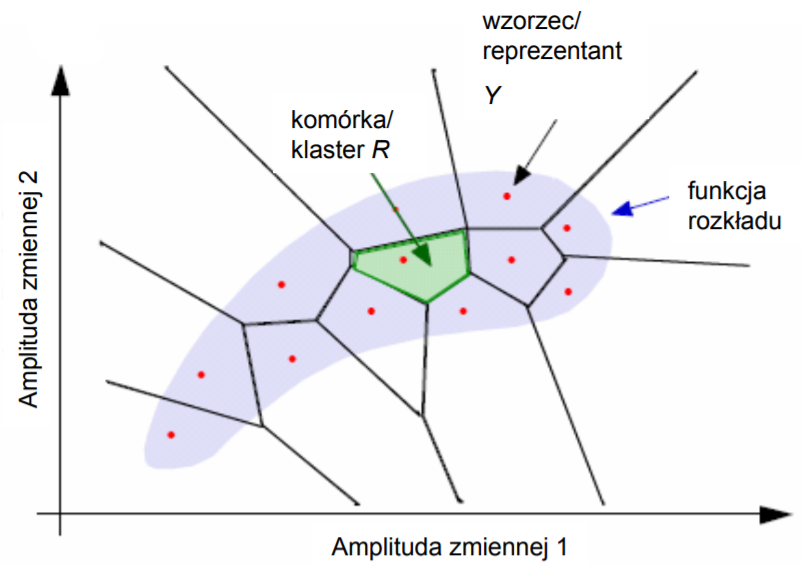
\includegraphics[width=0.6\textwidth]{images/kwantyzacja_wektorowa.png}
    \caption{Przykład podziału dwuwymiarowej przestrzeni danych na klastry grupujące według słownika. Źródło \cite{mwilczewski}}
    \label{fig:crossing}
\end{figure}

\subsection{Ogólny przebieg etapów pracy kwantyzatora wektorowego}

\begin{enumerate}
  \item Formowanie danych wejściowych do postaci \textit{N} wektorów \textit{n} - wymiarowych (etap wstępny). 
  \item Faza klasteryzacji: podział wszystkich wektorów wejściowych i konstrukcja książki kodowej (słownika) zawierającej \textit{K} najbardziej reprezentatywnych wektorów całego zbioru danych, tzw. wektorów kodowych. Konstrukcja książki kodowej może być wykonana w fazie wstępnej na podstawie zbioru treningowego lub dynamicznie we właściwej fazie kwantyzacji. Faza klasteryzacji jest kluczowym etapem kwantyzacji wektorowej.
  \item Faza indeksowania: przyporządkowanie każdemu wektorowi wejściowemu jednego wektora ze słownika i reprezentowanie wektora wejściowego indeksem słownika. 
\end{enumerate}

\begin{figure}[H]
    \centering
    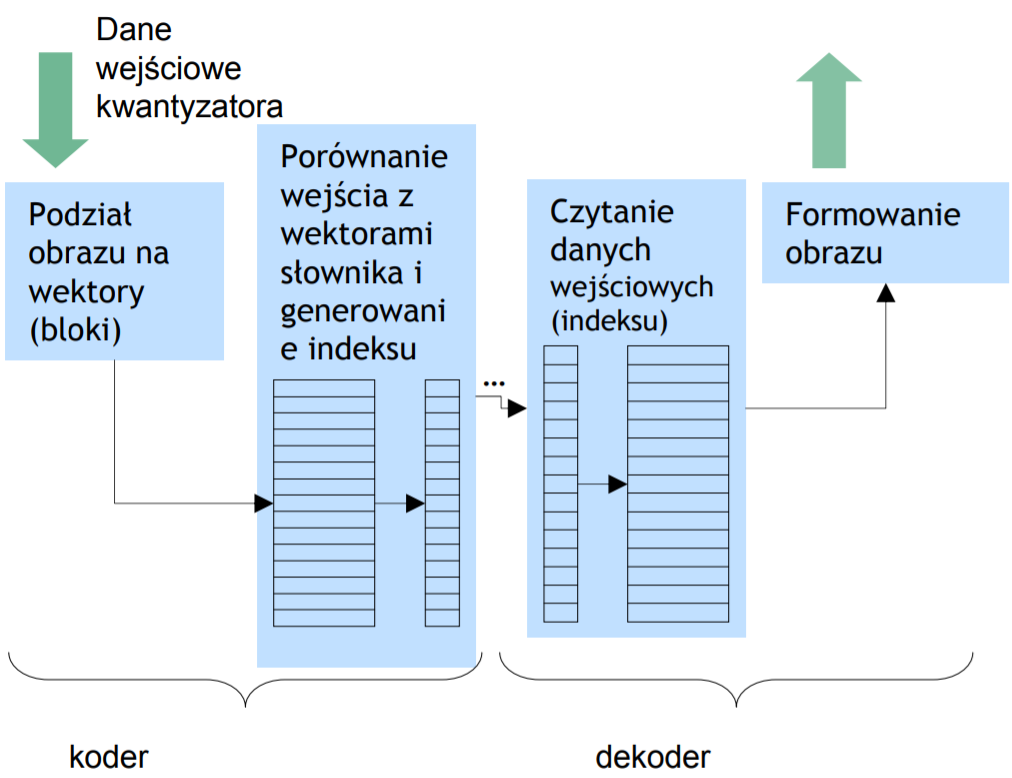
\includegraphics[width=0.6\textwidth]{images/schemat_kwantyzatora.png}
    \caption{Ogólny schemat pracy kwantyzatora. Źródło \cite{mwilczewski}}
    \label{fig:crossing}
\end{figure}

\begin{figure}[H]
    \centering
    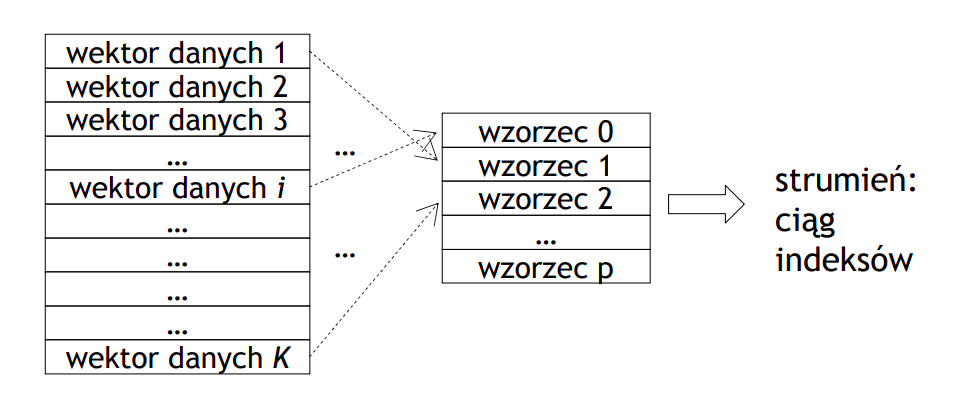
\includegraphics[width=0.6\textwidth]{images/wektory_danych.png}
    \caption{Porównywanie wektorów danych z wektorami ze słownika. Źródło \cite{mwilczewski}}
    \label{fig:crossing}
\end{figure}

Problemy jakie możemy napotkać podczas kwantyzacji wektorowej:
\begin{enumerate}
  \item Wybór odpowiedniej funkcji odległości w przestrzeni wektorowej.  
  \item Struktura książki kodowej (prosta struktura w postaci tablicy jest nieefektywna do przeglądania).
\end{enumerate}

\subsection{Inicjalizacja książki kodowej}

W procesie kwantyzacji wektorowej ważna rolę odgrywa postać książki kodowej ze względu na zbieżność do lokalnego minimum błędu kwantyzacji. Podstawowymi metodami inicjalizacji książki kodowej:

\begin{enumerate}
  \item metoda losowania,
  \item metoda grupowania najbliższych sąsiadów (ang. PNN - pairwise nearest neighbour)
  \item metoda rozdzielania (ang. splitting) 
\end{enumerate}

Pierwsza z wymienionych powyżej, czyli metoda losowa polega na wylosowaniu \textit{N} wektorów, gdzie \textit{N} jest liczba całkowitą. Oczywiście takie rozwiązanie jest odpowiednie, wtedy gdy nie mamy informacji na temat danych wektorowych. Posiadając informacje możemy wykorzystać ją do zawężenia obszaru losowego.

Druga metoda tworzenie słownika, czyli metoda grupowania pozwala osiągnąć lepsze wyniki niż metoda losowa, ale za to jest dużo bardziej czasochłonna. Polega ona na tworzeniu coraz liczniejszych grup zaczynając od jednoelementowej, związanej z każdym wektorem sekwencji. W następnych iteracjach wyznaczamy najbliższe grupy, czyli liczymy odległości pomiędzy środkami poszczególnych grup. Następnie dwie najbliższe sobie grupy zostają połączone tak aby zmniejszać liczbę grup.

Algorytm metody PNN:

\begin{enumerate}
 \item Rozważamy zestaw \textit{N} wektorów treningowych w przestrzeni euklidesowej \textit{K} - wymiarowej. Zadaniem konstrukcji książki kodowej jest odnalezienie zestawu wektorów kodowych \textit{M} poprzez minimalizacja średniej kwadratowej odległości \textit{M} pomiędzy wektorami treningowymi $T_{i}$ a ich
reprezentatywne wektory kodu $C_{j}$:

\begin{equation}
D = \frac{1}{N} \sum_{j=1}^M \sum_{T_{i}\in\mathbb{S_{j}}} ||T_{i} - C_{j}||^2
\end{equation}

\item Tutaj \textit{S={$S_{1}$,...,$S_{m}$}} definiuje grupowanie zestawu treningowego \textit{T}. Dla danego kodeksu \textit{C}. Optymalne grupowanie może być zbudowane poprzez przypisanie każdego wektora \textit{$T_{i}$} do klaster \textit{$j_{0}$} dla którego:

\begin{equation}
||T_{i} - C_{j0}||^2 = \displaystyle \min_{j_1,\dots ,M} ||T_{i} - C_{j}||^2
\end{equation}

\item Metoda ta rozpoczyna się od zainicjowania każdego wektor szkoleniowy \textit{$T_{i}$} jako własny klaster \textit{$S_{i}$}. Na każdym etapie algorytmu, dwa najbliższe klastry (\textit{$S_{a}$} i \textit{$S_{b}$}) są przeszukiwane i łączone. Odległość (koszt połączenia) \textit{d} pomiędzy dwoma klastrami jest definiowany jako wzrost zniekształcenia książki kodowej w przypadku połączenia klastrów:

\begin{equation}
d(S_{a}, S_{b}) = \frac{n_{a}n_{b}}{n_{a} + n_{b}} || C_{a} - C_{b} ||^2
\end{equation}

\item Wybrane klastry \textit{$S_{a}$} i \textit{$S_{b}$} są następnie łączone. Wielkość połączonego klastra \textit{$S_{a}$} + \textit{$S_{b}$} wynosi $n_{a+b}$=$n_{a}$+$n_{b}$, a odpowiednim wektorem kodu jest centroid wektorów szkoleniowych w klaster. Można go obliczyć jako średnią ważoną $C_{a}$ i $C_{b}$:

\begin{equation}
C_{a + b} = \frac{n_{a}C_{a} + n_{b}C_{b}}{n_{a} + n_{b}}
\end{equation}

\item Wystarczy zatem utrzymać tylko centroidy klastra $C_{i}$ i rozmiary klastrów $n_{i}$ w realizacji algorytmu. Proces łączenia jest powtarzany do momentu książka kodowa osiąga rozmiar \textit{M}. 

\end{enumerate}

gdzie:
\begin{itemize}[label=]
    \item \textit{T} - Zestaw \textit{N} wektorów treningowych $T = {[T_{1}, T_{2}, \dots, T_{N}]}$
    \item \textit{C} - Książka kodowa wektorów $C = {[C_{1}, C_{2}, \dots, C_{m}]}$
    \item \textit{M} - Rozmiar książki kodowej
    \item \textit{K} - Wymiar wektorów
    \item \textit{$S_{i}$} - Klaster (zestaw) wektorów treningowych $n_{i}$
    \item \textit{$NN_{i}$} - Indeksy najbliższego sąsiada klastra $S_{i}$
    \item \textit{$d_{i}$} - Zwiększenie zniekształcenia w przypadku połączenia klastrów $S_{i}$ i $NN_{i}$
    \item \textit{$R_{i}$} - Wskaźnik ważności. $R_{i}$ = true jeśli $d_{i}$ jest poprawne.
    \cite{tkaukoranta} 
\end{itemize}

Ostatnia wymieniona metoda jaką jest metoda rozdzielania - polega na szukaniu optymalnej książki. Konstrukcja rozpoczyna się od pojedynczego wektora – centroidu zbioru uczącego. W \textit{i} - tym kroku dokonywany jest (w drodze dodawania zaburzenia) podział każdego z wektorów kodowych na dwa wektory. Po takim rozdzieleniu uzyskana konfiguracja regionów decyzyjnych jest optymalizowana przez algorytm LBG, po czym dokonywany jest kolejny rozdział, etc.

\begin{figure}[H]
    \centering
    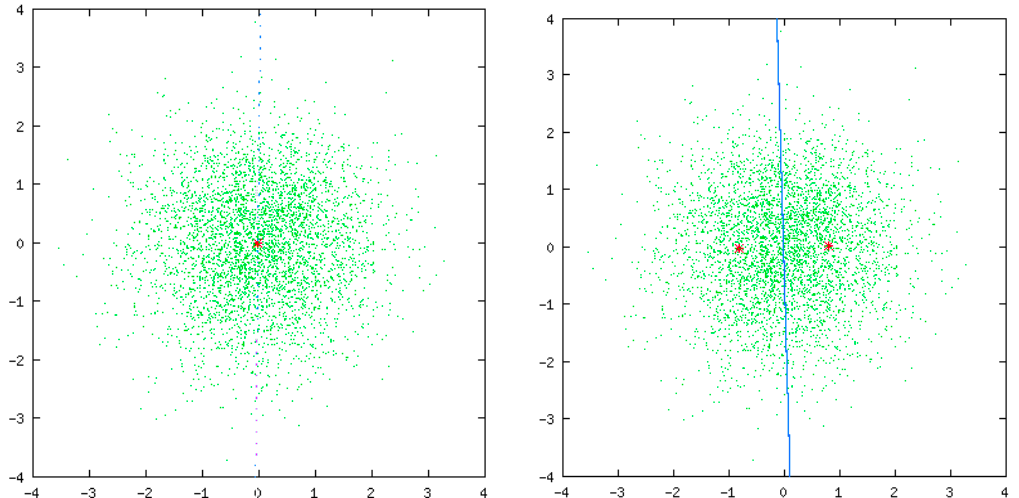
\includegraphics[width=0.6\textwidth]{images/rodzielania_1.png}
    \caption{Konstrukcja słownika metodą rozdzialania. Kolejne etapy konstrukcji wektorów kodowych (zaznaczone czerwonymi punktami) na zbiorze uczącym (zaznaczony kolorem zielonym).  Źródło \cite{mwilczewski}}
    \label{fig:crossing}
\end{figure}

\begin{figure}[H]
    \centering
    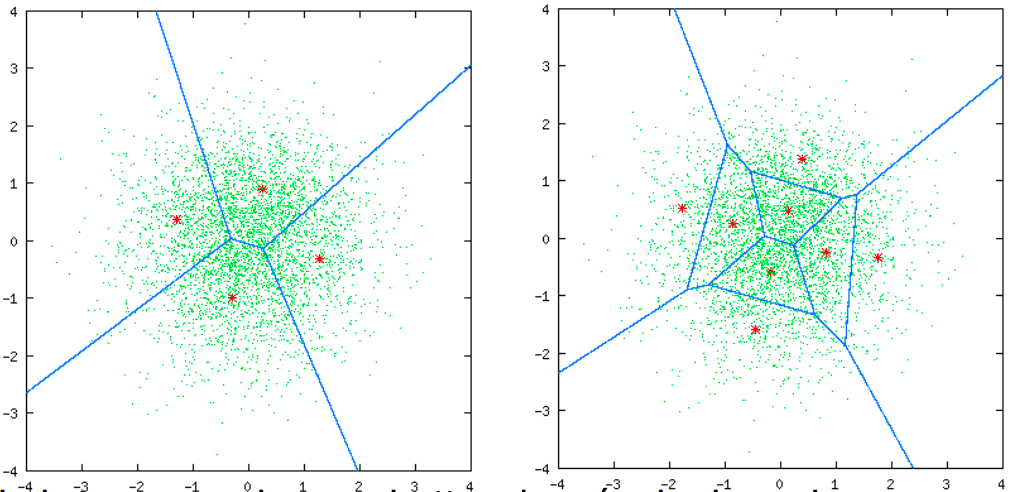
\includegraphics[width=0.6\textwidth]{images/rodzielania_2.png}
    \caption{Konstrukcja słownika metodą rozdzialania. Kolejne etapy konstrukcji wektorów kodowych (zaznaczone czerwonymi punktami) na zbiorze uczącym (zaznaczony kolorem zielonym).  Źródło \cite{mwilczewski}}
    \label{fig:crossing}
\end{figure}

\subsection{Algorytmy inicjalizowania słownika}

\subsubsection{Algorytm popularności}

Algorytm popularności jest prostym algorytmem generacji książki kodowej, który charakteryzuje się:

\begin{itemize}
  \item wektorami kodowymi staje się ustalona liczba wektorów danych najczęściej występujących w obrazie (konieczne jest ustalenie progu liczby wystąpień) 
  \item algorytm wyróżnia się stosunkowo małą złożonością obliczeniową i prostotą implementacji 
  \item wadą podstawowej wersji algorytmu popularności jest wprowadzanie do książki kodowej podobnych wartości (dominujących). Redukcję rozmiaru książki uzyskać można przez usunięcie bliskich (w sensie przyjętej metryki) wektorów i wprowadzenie kolejnych wektorów pod względem liczby wystąpień. 

\begin{figure}[H]
    \centering
    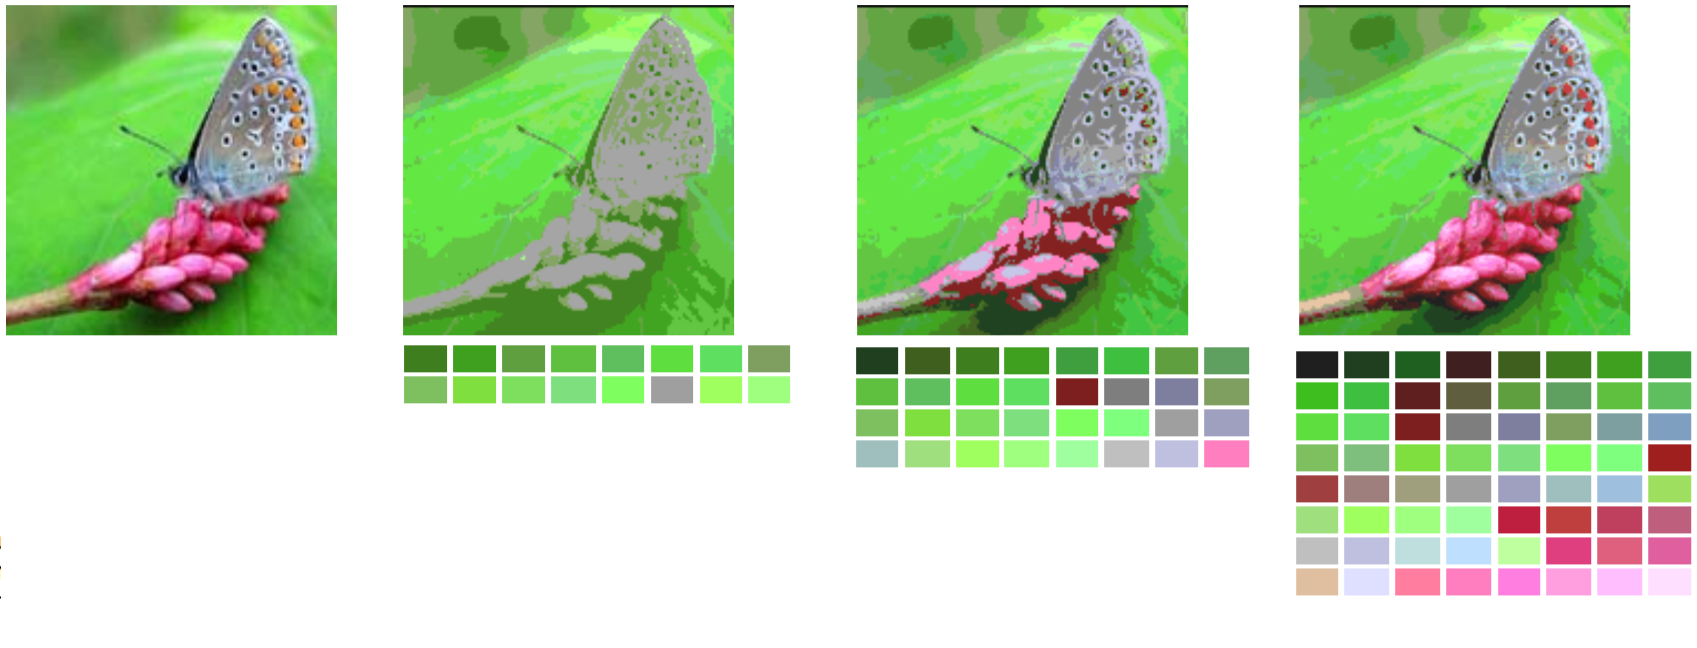
\includegraphics[width=0.6\textwidth]{images/motyle_2.png}
    \caption{Przykład kwantyzacji wektorowej przeprowadzonej z książką kodową skonstruowaną zgodnie z algorytmem popularności. Efekt kwantyzacji wektorowej z książkami kodowymi
rozmiaru odpowiednio: 16, 32 oraz 64. Źródło \cite{aprzelaskowski}}
    \label{fig:crossing}
\end{figure}
 
\end{itemize}

\subsubsection{Wektorowa kwantyzacja blokowa (BTC)}

Wektorowa kwantyzacja blokowa (BTC) charakteryzuje się:

\begin{itemize} 
\item W przypadku podstawowej wersji metody BTC każdy skwantyzowany blok obrazu reprezentowany jest jako strumień bitowy przez mapę bitową zawierającą $n^{2}$ bitów oraz dwa bajty reprezentujące poziomy rekonstrukcji. W takim przypadku:
     \begin{itemize}
        \item liczba wszystkich możliwych map bitowych jest równa $n^{2}$ = 65536,
        \item nie wszystkie z nich występują w każdym obrazie cyfrowym, np. ze względu na rozmiar obrazu oraz korelacje danych obrazowych, 
     \end{itemize}
\item jednym z możliwych sposobów wykorzystania powyższych obserwacji do kompresji obrazu jest kwantyzacja wektorowa map bitowych, tzn. reprezentacja zbioru wszystkich możliwych map bitowych przez niewielki jego podzbiór (słownik),
\item w fazie indeksowania, każda z map bitowych stworzonych dla kolejnych bloków obrazu porównywana jest ze zbiorem map w słowniku. Prostą miarą podobieństwa map jest liczba miejsc na których porównywane mapy różnią się. Mapą najbardziej podobną do zadanej jest mapą minimalizującą tak zdefiniowaną miarę,
\item wykorzystanie zbioru map stanowiących słownik zwiększa stopień kompresji. Przykład: w przypadku bloków 4x4 oraz 32 elementowego słownika 16 bitów reprezentujących elementy oryginalnej mapy można zastąpić 5 bitowym indeksem słownika. Zwiększa to stopień kompresji z CR=4.0 do CR=6.09.
\end{itemize}

\subsection{Algorytmy budowy słownika}

\subsubsection{Algorytm Lindego-Buza-Graya}

Algorytm Lindego-Buza-Graya (LBG), powstał 1980, służy od do generowania książki kodowej. Przebieg algorytmu przedstawia się następująco:

\begin{itemize} 
\item określić wektory danych zbioru uczącego. Spośród wszystkich \textit{N} wektorów wejściowych wybierz losowo \textit{K} wektorów stanowiących wstępną wersję słownika,
\item korzystając z metryki euklidesowej, \textit{d(X,Y)}, dokonaj klasteryzacji wektorów danych wokół słów kodowych bieżącej wersji słownika
     \begin{itemize}
        \item bierzemy każdy kwadrat z obrazu o rozmiarze \textit{(4x4)} i sprawdzamy, któremu reprezentantowi ze słownika jest najbliżej do 
        naszego kwadratu, każdy piksel wewnątrz tego kwadratu porównujemy ze sobą i liczymy ich różnice w kwadracie 
        \todo{Sprawdzić czy wzór został poprawnie zapisany}:
        
		\begin{equation}
		d(B_{m}, C_{i}) < d(B_{m}, C_{j})
		\end{equation}
		
		gdzie:
		\begin{itemize}[label=]
    		\item $B_{m}$ - block obrazu,
    		\item $C_{i}$ - słowo kodowe ze słownika
    		\item $C_{j}$ - kolejne słowo kodowe ze słownika
		\end{itemize}	        
        
        \item następnie sumujemy różnicę 16 kwadratów
        \item sprawdzamy kwadrat obrazu z każdym reprezentantem słownika centroid
        \item przypisujemy wybrany kwadrat do reprezentanta słownika
     \end{itemize}
\item wyznaczamy globalny błąd kwantyzacji popełniony w bieżącej iteracji czyli wykonujemy sumowanie wszystkich znalezionych odległości miedzy poszczególnymi kwadratami a centroidami 
 
\begin{equation}
e = \sum_{i=1}^K \sum_{x\in\mathbb{R}} d(X, Y_{i}) 
\end{equation}

\item sprawdzić czy popełniany błąd zmienił się względem poprzedniej iteracji jeśli nie ma to kończymy algorytm (dla uproszczenia ustaliliśmy, że liczbę iteracji będzie podawana z ręki)
\item wyznacz centroidy każdego regionu decyzyjnego i uczyń je wektorami kodowymi kolejnej iteracji słownika. Przejdź do kroku 2. 
\end{itemize}
 
Problemy tego algorytmu:

\begin{itemize}
	\item wrażliwość na inicjalną postać książki kodowej 
	\item problem pustych przedziałów 
\end{itemize}

\todo{Sparametryzowany wzór pliku wynikowego}

\subsubsection{Kwantyzacja wektorowa z usuniętą średnią}

Kwantyzacja wektorowa z usuniętą średnią (MRVQ) jest zmodyfikowaną wersją schematu VQ. Celem MRVQ jest zapewnienie lepszej jakości obrazu niż VQ. Aby osiągnąć ten cel, do kodowania każdego bloku obrazu w MRVQ wykorzystuje się wartość średnią bloku oraz indeks wektora resztkowego. Schemat MRVQ składa się z trzech procedur: generowania książki kodów resztkowych, kodowania obrazu i dekodowania obrazu. Aby wygenerować resztkową książkę kodową RCB z N resztkowych słów kodowych dla MRVQ, zastosowano algorytm LBG. Zamiast obrazów szkoleniowych używanych do projektowania książki kodowej VQ, do projektowania książki kodowej MRVQ wykorzystuje się wektory resztkowe. Po pierwsze, bloki obrazów treningowych są generowane przez podzielenie obrazów treningowych na nienakładające się na siebie bloki obrazów o $4 \times 4$ pikseli. Każdy blok obrazów treningowych składający się z $4 \times 4$ pikseli może być postrzegany jako wektor \textit{k} -wymiarowy, gdzie \textit{k} = $4 \times 4$. Każdy wektor treningu jest przekształcany na jeden wektor reprezentowany poprzez odjęcie jego średniej wartości bloku od wartości każdego piksela. Następnie algorytm LBG opisany w sekcji 2.5.1 jest wykorzystywany do projektowania książki kodów resztkowych RCB = ( $rcw_{0}$, $rcw_{1}$, \dots , , $rcw_{N-1}$ ) przy użyciu wektorów resztkowych.

Wartość średnia bloku \textit{bm} dla każdego bloku obrazu \textit{x} jest obliczana za pomocą wyrażenia: 

\begin{equation}
bm = \frac{1}{k} \sum_{i=0}^{k-1} x_{i}
\end{equation}

Następnie generowany jest pozostały wektor \textit{rv} poprzez odjęcie wartości \textit{bm} od każdej wartości piksela w \textit{x}. Przeszukiwane jest najbliższe pozostałe słowo kodowe w \textit{RCB} dla pozostałego wektora \textit{rv} i zapisywany jest indeks najbliższego pozostałego słowa kodowego.\cite{meanremovedVQ} 

\todo{Sparametryzowany wzór na długość pliku wynikowego}

\subsection{Wykorzystywane metryki}

\subsubsection{PSNR}

Szczytowy stosunek sygnału do szumu, (ang. peak signal-to-noise ratio ( PSNR)) – stosunek maksymalnej mocy sygnału do mocy szumu zakłócającego ten sygnał.  

Najczęściej PSNR stosowany jest do oceny jakości kodeków wykorzystujących stratną kompresję obrazków. W takim przypadku sygnałem są nieskompresowane dane źródłowe, a szumem – artefakty (zniekształcenia) spowodowane zastosowaniem kompresji stratnej. 

W celu wyznaczenie PSNR, należy najpierw obliczyć współczynnik MSE (błąd średniokwadratowy) bazując na obu porównywanych obrazkach za pomocą wzoru:

\begin{equation}
MSE = \frac{1}{N \cdot M} \sum_{i=1}^N \sum_{j=1}^M ([f(i, j) - f^{'}(i, j)]^2
\end{equation}

gdzie:
\begin{itemize}[label=]
    \item $N, M$ - wymiary obrazu w pikselach,
    \item $f(i, j)$ - wartość piksela o współrzędnych $i(i, j)$ obrazu oryginalnego
    \item $f^{'}(i, j)$ - wartość piksela o współrzędnych $i(i, j)$ obrazu skompresowanego
\end{itemize}

Następnie wyliczoną wartość MSE należy podstawić do końcowego wzoru: 

\begin{equation}
PSNR = 10 \cdot \log_10 \frac{[max(f(i,j))]^2}{MSE}
\end{equation}

gdzie:
\begin{itemize}[label=]
    \item $max(f(i,j))$ - wartość maksymalna danego sygnału; w przypadku obrazów zwykle jest to wartość stała, np. dla obrazów monochromatycznych o reprezentacji 8-bitowej wynosi 255.
\end{itemize}

\subsubsection{SSIM}

Podobieństwo strukturalne miarą indeksu \textit{(ang. structural similarity index measure)} jest to metoda, która służy 
do pomiaru podobieństwa między dwoma obrazami. Indeks \textit{SSIM} to pomiar jakości obrazu bazowego (nieskompresowanego) 
do obrazu po przekształceniach. SSIM to model oparty na percepcji, który traktuje degradację obrazu jako postrzeganą zmianę
w informacjach strukturalnych, przy jednoczesnym uwzględnieniu ważnych zjawisk percepcyjnych, w tym zarówno terminów maskowania 
luminancji, jak i maskowania kontrastu. Różnica w stosunku do innych technik, takich jak \textit{MSE} lub \textit{PSNR},
polega na tym, że te podejścia szacują błędy bezwzględne. Idea informacji strukturalnych polega na tym, że piksele mają silne współzależności,
zwłaszcza gdy są znajdują się blisko siebie w przestrzenni. Zależności te niosą ważne informacje o strukturze obiektów \mbox{na scenie wizualnej \cite{channappayya2008rate}.}

Algorytm SSIM:

\begin{equation}
SSIM(x, y) = \frac{(2\mu_{x}\mu_{y} + c_{1}) (2\delta_{xy} + c_2)}{(\mu_{x}^2 + \mu_{y}^2 + c_{1}) (\delta_{x}^2 + \delta_{x}^2 + c_2)}
\end{equation}

gdzie:
\begin{itemize}[label=]
    \item $\mu_{x}$ - średnia x
    \item $\mu_{y}$ - średnia y
    \item $\delta_{x}^2$ - odchylenie od x
    \item $\delta_{y}^2$ - odchylenie od y
    \item $\delta_{xy}$ - kowariancja x i y
\end{itemize}

\subsubsection{FSIM}

\todo{Opisać FSIM}

\subsubsection{CR}

\subsubsection{RMSE}

Podstawowy błąd średniokwadratowy (RMSE) - jest to reguła, która mierzy średnią wielkość błędu. Jest to pierwiastek kwadratowy każdej różnicy między prognozowaną a odpowiadającą jej wartościom, podniesiona do kwadratu, a następnie uśredniona w próbie. Ponieważ błędy są podnoszone do kwadratu, zanim zostaną uśrednione, sprawia to, że RMSE nadaje stosunkowo dużą wagę dużym błędom. Oznacza to, że RMSE jest najbardziej przydatny, gdy duże błędy są szczególnie niepożądane.

Wzór RMSE:

\begin{equation}
RMSE = \sqrt{\frac{1}{n} \sum_{j=1}{n} (y_{j} - \hat{y_{j}} )^2}
\end{equation}

gdzie:
\begin{itemize}[label=]
    \item $n$ - średnia próby
    \item $y_{j}$ - prognozowana wartość błędu
    \item $\hat{y_{j}}$ - rzeczywista wartość błędu\cite{rmse}
\end{itemize}

\section{Badania}

\subsection{Algorytm LBG z losową inicjalizacją słownika}

Przeprowadzono badania na wszystkich dostarczonych obrazach badawczych. Kwantyzację przeprowadzono na blokach o rozmiarach $4 \times 4$ oraz dla książki
kodowej o długości $512$ elementów. Dane zebrano w \mbox{tablicy \ref{tab:lbg_random}} i podsumowano w tablicy \mbox{\ref{tab:lbg_summary}}.

% Please add the following required packages to your document preamble:
% \usepackage{booktabs}
\begin{table}[h]
\centering
\begin{tabular}{@{}lrrrr@{}}
\toprule
Obraz              & PSNR {[}dB{]} & SSIM   & MSE      & NRMSE  \\ \midrule
Aerial.bmp         & 31.6636       & 0.8747 & 137.5262 & 0.0634 \\
airfield.bmp       & 30.8671       & 0.7938 & 156.1186 & 0.0804 \\
airplane.bmp       & 34.6427       & 0.9236 & 49.7802  & 0.0382 \\
baboonTMW.bmp      & 29.9951       & 0.7893 & 219.1716 & 0.1089 \\
balloon.bmp        & 39.3125       & 0.9533 & 10.6350  & 0.0292 \\
balloon\_noise.bmp & 39.1234       & 0.9496 & 11.2513  & 0.0302 \\
BARB.bmp           & 32.2852       & 0.8837 & 89.9736  & 0.0790 \\
BARB2.bmp          & 32.1664       & 0.8853 & 89.5440  & 0.0754 \\
barb512.bmp        & 32.1491       & 0.8806 & 95.2525  & 0.0754 \\
BOARD.bmp          & 36.4226       & 0.9313 & 28.9137  & 0.0459 \\
boat512.bmp        & 32.8108       & 0.8650 & 71.7116  & 0.0614 \\
boats.bmp          & 34.3485       & 0.9128 & 43.6047  & 0.0509 \\
bridge.bmp         & 30.3832       & 0.8038 & 157.6636 & 0.0994 \\
bridge256.bmp      & 30.3125       & 0.8323 & 141.0575 & 0.0946 \\
camera256.bmp      & 33.7937       & 0.9055 & 94.8728  & 0.0726 \\
couple.bmp         & 32.4539       & 0.8631 & 74.4537  & 0.0670 \\
couple256.bmp      & 35.5769       & 0.9339 & 29.8176  & 0.1196 \\
crowd512.bmp       & 33.4139       & 0.9171 & 64.5795  & 0.0815 \\
EARTH.bmp          & 33.5174       & 0.9325 & 65.9923  & 0.0842 \\
elaine.bmp         & 33.1995       & 0.8364 & 40.8950  & 0.0444 \\
ELIF.bmp           & 37.8132       & 0.9587 & 16.7079  & 0.0544 \\
finger.bmp         & 29.9399       & 0.9008 & 131.6425 & 0.0925 \\
FROG512.BMP        & 29.8664       & 0.7281 & 168.3580 & 0.1013 \\
GIRL.bmp           & 35.2442       & 0.9169 & 26.8099  & 0.0367 \\
GOLD.bmp           & 33.3489       & 0.8668 & 45.4286  & 0.0589 \\
GOLDHILL.BMP       & 32.9129       & 0.8629 & 52.1809  & 0.0590 \\
harbour512.bmp     & 32.2399       & 0.8563 & 127.0800 & 0.0854 \\
HOTEL.bmp          & 33.3766       & 0.8960 & 67.1312  & 0.0753 \\
lax512.bmp         & 30.9269       & 0.7800 & 160.8272 & 0.1421 \\
lenaTMW.bmp        & 33.6248       & 0.8704 & 52.2250  & 0.0644 \\
lennagrey.bmp      & 34.6031       & 0.8994 & 39.0316  & 0.0471 \\
man512.bmp         & 33.0232       & 0.8705 & 64.1381  & 0.0660 \\
noisesquare.bmp    & 32.9291       & 0.8254 & 35.6925  & 0.0311 \\
OMAHA.bmp          & 29.9031       & 0.8378 & 327.2889 & 0.1044 \\
peppersTMW.bmp     & 34.2263       & 0.8743 & 42.6578  & 0.0497 \\
SAILBOAT.bmp       & 32.9982       & 0.8771 & 64.4069  & 0.0592 \\
seismic.bmp        & 39.9778       & 0.9726 & 7.4695   & 0.0213 \\
SENA.bmp           & 37.5456       & 0.9542 & 15.2120  & 0.0435 \\
SENSIN.bmp         & 35.3720       & 0.9468 & 23.9566  & 0.0455 \\
shapes.bmp         & 38.4559       & 0.9612 & 22.2232  & 0.0534 \\
SINAN.bmp          & 36.5850       & 0.9493 & 18.1502  & 0.0325 \\
Tank512.bmp        & 33.6339       & 0.8500 & 37.7513  & 0.0455 \\
Truck512.bmp       & 33.9556       & 0.8830 & 33.5212  & 0.0524 \\
woman1.bmp         & 33.3459       & 0.8616 & 65.1471  & 0.0570 \\
woman2.bmp         & 37.7312       & 0.9416 & 13.1210  & 0.0292 \\
ZELDA.bmp          & 36.5893       & 0.9163 & 18.5568  & 0.0368 \\ \bottomrule
\end{tabular}
\caption{Porównanie jakości kwantyzacji algorytmu budowy słownika LBG z losową inicjalizacją słownika dla bloku $4 \times 4$ oraz długości słownika $512$.}
\label{tab:lbg_random}
\end{table}

% Please add the following required packages to your document preamble:
% \usepackage{booktabs}
\begin{table}[H]
\centering
\begin{tabular}{@{}lrrrr@{}}
\toprule
         & PSNR {[}dB{]} & SSIM  & MSE     & NRMSE \\ \midrule
Minimum  & 29.8664       & 0.7281 & 7.4695   & 0.0213 \\
Maksimum & 39.9778       & 0.9726 & 327.2889 & 0.1421 \\
Średnia  & 33.8828       & 0.8853 & 72.8159  & 0.0641 \\ \bottomrule
\end{tabular}
\caption{Przedstawienie wartości minimalnej, maksymalnej oraz uśrednienie wyników dla poszczególnych metryk}
\label{tab:lbg_summary}
\end{table}

\subsubsection{Wyznaczenie optymalnej liczby iteracji w algorytmie budowy słownika LBG}

\todo{Opisać jak wyznaczono optymalną liczbę iteracji oraz wnioski}

\begin{figure}[H]
\centering
  \centering
  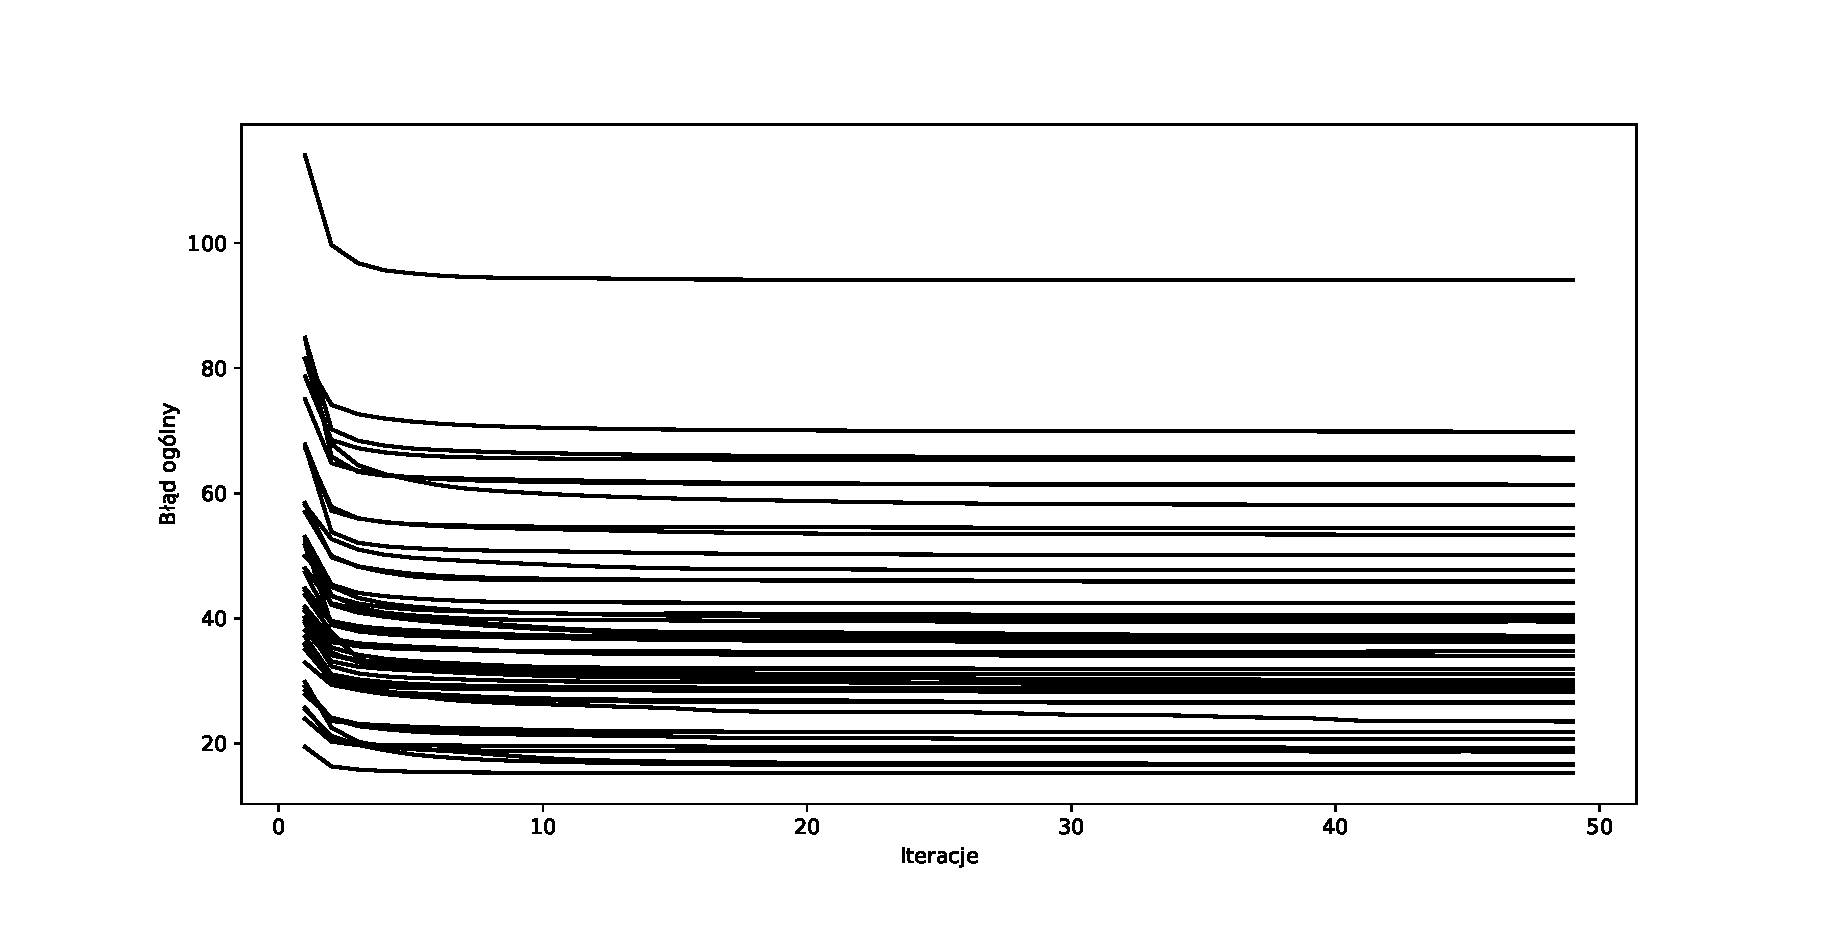
\includegraphics[width=.9\linewidth]{images/lbg_4x4_32_50_iterations.eps}  
  \caption{\todo{Opis wykresu (każda linia to jeden obraz).}}
  \label{fig:lbg_iterations}
\end{figure}

\begin{figure}[H]
  \centering
  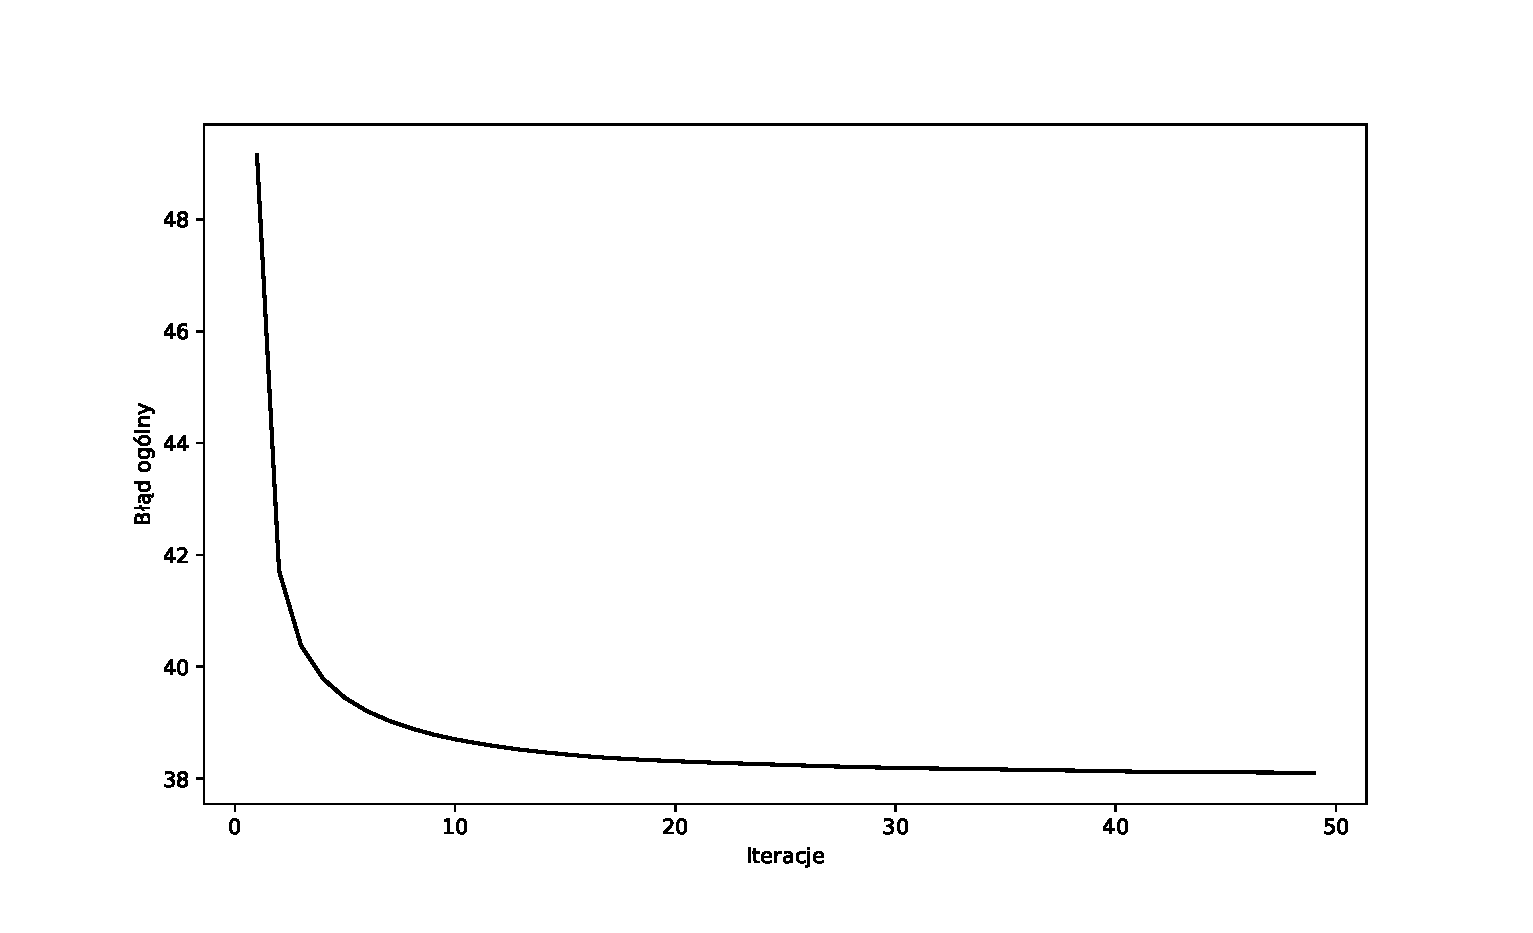
\includegraphics[width=.9\linewidth]{images/lbg_4x4_32_mean_iterations.eps}  
  \caption{\todo{Opis wykresu (średnia z wszystkich obrazów).}}
  \label{fig:lbg_iterations_mean}
\end{figure}


\FloatBarrier
\section{Podsumowanie}

\lipsum[1-3]

\bibliographystyle{unsrt}  
\bibliography{references}  %%% Remove comment to use the external .bib file (using bibtex).
%% and comment out the ``thebibliography'' section.

\end{document}